\documentclass{article}
\usepackage{arxiv}

\usepackage[utf8]{inputenc}
\usepackage[english, russian]{babel}
\usepackage[T1]{fontenc}
\usepackage{url}
\usepackage{booktabs}
\usepackage{amsfonts}
\usepackage{nicefrac}
\usepackage{microtype}
\usepackage{lipsum}
\usepackage{graphicx}
\usepackage{natbib}
\usepackage{doi}
\usepackage{amsmath}



\title{Классификация на основе риманновой геометрии и метрики лапласиана для ИМК}

\author{ Парвиз~Каримов\\%\thanks{Use footnote for providing further
		% information about author (webpage, alternative
		% address)---\emph{not} for acknowledging funding agencies.} \\
	% Department of Computer Science\\
	% Cranberry-Lemon University\\
	% Pittsburgh, PA 15213 \\
	\texttt{karimov.pd@phystech.edu} \\
	%% examples of more authors
	\And
	Валентина~Смит \\
	% Department of Electrical Engineering\\
	% Mount-Sheikh University\\
	% Santa Narimana, Levand \\
	\texttt{smit.vi@phystech.edu} \\
	\And
	Георгий~Жаров\\
	% Affiliation \\
	% Address \\
	\texttt{zharov.g@phystech.edu} \\
	%% \And
	%% Coauthor \\
	%% Affiliation \\
	%% Address \\
	%% \texttt{email} \\
	%% \And
	%% Coauthor \\
	%% Affiliation \\
	%% Address \\
	%% \texttt{email} \\
}
% \date{31.12.2023}

% \renewcommand{\shorttitle}{\textit{arXiv} Template}
\renewcommand{\shorttitle}{Классификация EEG на основе римановой геометрии и метрики лапласиана для ИМК}
%%% Add PDF metadata to help others organize their library
%%% Once the PDF is generated, you can check the metadata with
%%% $ pdfinfo template.pdf
\hypersetup{
pdftitle={Классификация EEG на основе римановой геометрии и метрики лапласиана для ИМК},
pdfsubject={q-bio.NC, q-bio.QM},
pdfauthor={Парвиз~Каримов, Валентина~Смит, Георгий~Жаров},
pdfkeywords={Riemannian Geometry, Graph Laplacian, BCI, EEG classification},
}

\begin{document}
\maketitle

\begin{abstract}
	Работа посвящена мультиклассовой классификации данных для интерфейса мозг-компьютер на основе данных электроэнцефалограмм на основе модели с применением римановой геометрии, метрики лапласиана и матрицы внимания.
\end{abstract}


\keywords{Riemannian Geometry, Graph Laplacian, BCI, EEG classification}

\section{Введение}
В данном исследовании предлагается рассмотреть пространственно-временную модель визуализации
временного ряда данных электроэнцефалограммы (\textit{EEG}) для предсказания на основе фрагмента \textbf{EEG} видео. При просмотре видео в интернете наш мозг определённым образом реагирует на это, что возбуждает разные его отделы. Например, задний отдел реагирует на мимику человека. Или, как другой пример, мозг среднестатистического человека реагирует на зрительные раздражения. \textit{EEG} позволяет определить активность мозга в тот или иной момент времени в определённых участках, так при влиянии раздражителей мы можем выявить зависимость реакции конкретной части головного мозга.
\par
Основной целью работы является разработка модели классификации данных временного ряда с предобработкой данных на основе римановой геометрии, метрики лапласиана и матрицы внимания.
\par
Предметом исследования являются данные интракраниальной электроэнцефалографии (iEEG)\cite{data2022}, полученные непосредственно от электродов, установленных на поверхности мозга пациентов. Это позволило исследователям получить данные с высокой степенью пространственного и временного разрешения, что критически важно для изучения детальных паттернов мозговой активности. В ходе исследования использовались системы регистрации с частотой дискретизации $512$Гц или $2048$Гц, что обусловлено различиями в клинических системах, применяемых в различных медицинских учреждениях.
\par
В данной области основной проблемой является решение трудностей с большой размерностью данных.
В ряде статей \cite{BARACHANT2013172, barachant2012} предлагается применение модели декодера для многомерных наблюдений, пользуясь средствами римановой геометрии. Авторы изучают когнитивные процессы, которые в свою очередь тоже являются многомерным временным рядом. Целесообразность применения описанных в этих статьях методов описана, например, в статье \cite{Congedo2017}, более того, в статье даётся объяснение тому, почему в данной области не применяются классические методы для решения задачи декодирования \textit{EEG}-сигнала.
\par
В статье \cite{PP2014} рассматривается подход к классификации некалиброванных данных \textit{EEG} с применением римановой геометрии. Предлагается подход для построения матриц ковариации путём конкатенации среднего и отдельной попытки, что позволяет учесть временную структуру и уменьшить размерность временных данных.
\par
В \cite{GRAND2021} рассматривается новый подход обучения на основе графовых нейронных сетей, как непрерывный процесс дифузии с применением механизма внимания, что даёт устойчивость модели к шумам в данных.
\par
Декодирование \textit{EEG}-сигналов является востребованной задачей. Важность этой задачи обосновывается возможностями, которые могут появиться у людей с ограниченными возможностями - речь идёт про протезы, которые смогут полноценно мимикрировать под потерянную часть тела. Другим применением можно назвать сферу развлечений, в которой в последнее время достаточно популярны технологии виртуальной (VR) и дополненной (AR) реальности.

\section{Обозначения}
\label{sec:headings Обозначения}
	Введем следующие обозначения:
	\begin{itemize}
		\item $x$ -- сэмпл данных EEG, поступающий на вход
		\item $y$ -- истинная метка класса.
	\end{itemize}

\section{Постановка задачи}
\label{sec:headings Постановка}
Пусть на вход получаем матрицу данных ЭЭГ 
\begin{equation}
\bm{E} = \begin{bmatrix}
e_{11} & e_{12} & \cdots & e_{1f} \\
e_{21} & e_{22} & \cdots & e_{2f} \\
\vdots & \vdots & \ddots & \vdots \\
e_{n1} & e_{n2} & \cdots & e_{nf}
\end{bmatrix}  \in {\mathbb{R}^{n \times f}^T},
\end{equation}
 где $n$ --- количество электродов, $f$ --- частота измерения.
 \par
 Требуется найти модель классификации $f: \mathbb{R}^{n \times f} \rightarrow Y$ между сегментами ${E}$ метками класса конечного множества $Y$.\\

 

% See Section \ref{sec:headings}.

% \subsection{Headings: second level}
% \lipsum[5]
% \begin{equation}
% 	\xi _{ij}(t)=P(x_{t}=i,x_{t+1}=j|y,v,w;\theta)= {\frac {\alpha _{i}(t)a^{w_t}_{ij}\beta _{j}(t+1)b^{v_{t+1}}_{j}(y_{t+1})}{\sum _{i=1}^{N} \sum _{j=1}^{N} \alpha _{i}(t)a^{w_t}_{ij}\beta _{j}(t+1)b^{v_{t+1}}_{j}(y_{t+1})}}
% \end{equation}

% \subsubsection{Headings: third level}
% \lipsum[6]

% \paragraph{Paragraph}
% \lipsum[7]



% \section{Examples of citations, figures, tables, references}
% \label{sec:others}

% \subsection{Citations}
% Citations use \verb+natbib+. The documentation may be found at
% \begin{center}
% 	\url{http://mirrors.ctan.org/macros/latex/contrib/natbib/natnotes.pdf}
% \end{center}

% Here is an example usage of the two main commands (\verb+citet+ and \verb+citep+): Some people thought a thing \citep{kour2014real, hadash2018estimate} but other people thought something else \citep{kour2014fast}. Many people have speculated that if we knew exactly why \citet{kour2014fast} thought this\dots

% \subsection{Figures}
% \lipsum[10]
% See Figure \ref{fig:fig1}. Here is how you add footnotes. \footnote{Sample of the first footnote.}
% \lipsum[11]

% \begin{figure}
% 	\centering
% 	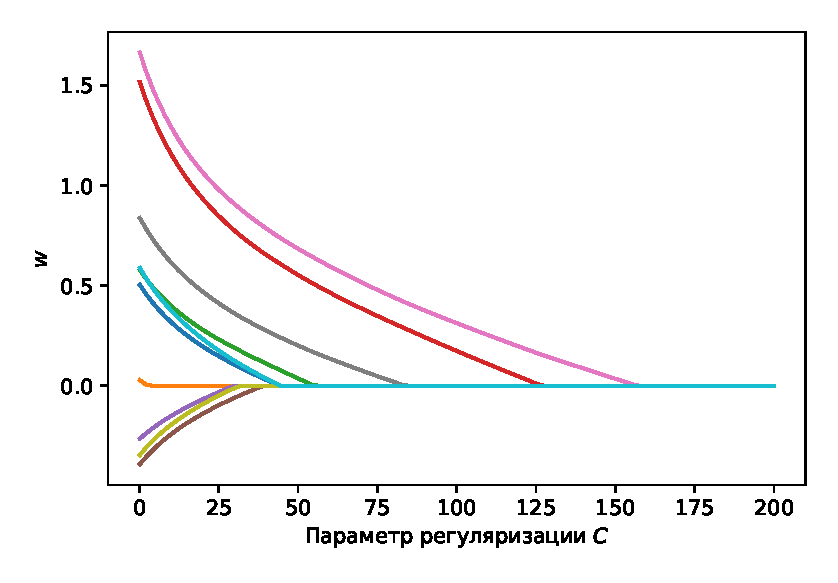
\includegraphics[width=0.5\textwidth]{../figures/log_reg_cs_exp.eps}
% 	\caption{Sample figure caption.}
% 	\label{fig:fig1}
% \end{figure}

% \subsection{Tables}
% See awesome Table~\ref{tab:table}.

% The documentation for \verb+booktabs+ (`Publication quality tables in LaTeX') is available from:
% \begin{center}
% 	\url{https://www.ctan.org/pkg/booktabs}
% \end{center}


% \begin{table}
% 	\caption{Sample table title}
% 	\centering
% 	\begin{tabular}{lll}
% 		\toprule
% 		\multicolumn{2}{c}{Part}                   \\
% 		\cmidrule(r){1-2}
% 		Name     & Description     & Size ($\mu$m) \\
% 		\midrule
% 		Dendrite & Input terminal  & $\sim$100     \\
% 		Axon     & Output terminal & $\sim$10      \\
% 		Soma     & Cell body       & up to $10^6$  \\
% 		\bottomrule
% 	\end{tabular}
% 	\label{tab:table}
% \end{table}

% \subsection{Lists}
% \begin{itemize}
% 	\item Lorem ipsum dolor sit amet
% 	\item consectetur adipiscing elit.
% 	\item Aliquam dignissim blandit est, in dictum tortor gravida eget. In ac rutrum magna.
% \end{itemize}


\bibliographystyle{unsrtnat}
\bibliography{references}

\end{document}